\documentclass[12pt]{article}
\usepackage[utf8]{inputenc}
\usepackage[margin=1in]{geometry}
\usepackage{hyperref,indentfirst,amstext,amsmath,amssymb,amsthm,esint,float,graphicx,caption}

\usepackage[hyperref=true,backref=true,sorting=none]{biblatex}
\hypersetup{colorlinks=true,linkcolor=red,citecolor=red,urlcolor=blue}
\addbibresource{main.bib}
\renewcommand*{\bibfont}{\small}

\let\Pr\relax
\DeclareMathOperator*{\Pr}{\mathbb{P}}
\DeclareMathOperator*{\E}{\mathbb{E}}
\graphicspath{{./graphs/}}

\parindent 0.3in
\title{Multi-Armed Bandit Learning}
\author{James Heppenstall, Haochen Li, Alberto Mizrahi}
\date{7 May 2019}

\begin{document}
\maketitle

\section{Introduction}

In this project, we focus on two formalizations of the multi-armed bandit problem: \textbf{stochastic iid rewards} and \textbf{adversarial rewards}. For the former, we survey epsilon strategies, UCB strategies, and Thompson sampling. For the latter, we survey the Exp3 and Exp3.P algorithms. In particular, we experimentally verify their regret bounds and compare their performance on real-world data, specifically that of the stock market over the past ten years. We finally try to motivate the problem in the broader context of Princeton's Theoretical Machine Learning (COS 511) course.

At a high level, the multi-armed bandit problem is a sequential decision problem concerned with how one dynamically allocates a resource among a set of actions to maximize some cumulative reward \cite{robbins1952}. While the original motivation for this problem came from clinical trials \cite{thompson1933}, the term ``multi-armed bandit" actually traces back to slot machines, each colloquially referred to as a ``one-armed bandit", by virtue of the arm one pulls down and the fact that they often empty gamblers' pockets. It should come as no surprise that Gittins' canonical example therefore considers a gambler who must decide which arm to pull among $K$ non-identical slot machines in order to maximize his return \cite{gittins1979}.

The multi-armed bandit learning problem has received much attention, particularly in the reinforcement learning community, because it touches upon the intrinsic tradeoff between \textbf{exploration} and \textbf{exploitation} in sequential experiments \cite{bubeck2012}. In the context of Gittins' slot machines, should one \textit{explore} slot machines with unknown rewards or \textit{exploit} the slot machine believed to give the highest reward? Every algorithm we survey approaches this fundamental question in a different manner, yielding varying theoretical guarantees and empirical results.

\section{Theoretical Background}

\subsection{Notation and Terminology}

We adopt Bubeck and Cesa-Bianchi's notation and terminology to formulate the multi-armed bandit problem \cite{bubeck2012}. Let the agent implementing some bandit strategy be the player. Assume there are $K\geq 2$ arms and $T\geq K$ rounds, both \textit{known} to the player. Each arm $i=1,...,K$ is associated with a sequence $X_{i,1},...,X_{i,T}$ of \textit{unknown} rewards. Every round $t=1,...,T$, the player selects an arm $I_{t}\in\{1,...,K\}$ and receives the reward $X_{I_{t},t}$. The goal is to maximize the player's cumulative reward $\sum_{t=1}^{T}X_{I_{t},t}$.

In the stochastic iid reward setting, each arm $i$ is associated with a probability distribution $\nu_{1},...,\nu_{K}$ that remains identical throughout. Every round $t$, the reward $X_{I_{t},t}\sim\nu_{I_{t}}$ is drawn independently of past player actions. In the adversarial reward setting, an adversary defines a gain vector $g_{t}=(g_{1,t},...,g_{K,t})$ at the beginning of every round $t$. The player then selects arm $I_{t}$ and receives the reward $X_{I_{t},t}=g_{I_{t},t}$ without observing the gains of other arms. Note that stochastic iid rewards are a strict subset of adversarial rewards where the gain vector in round $t$ is defined according to random draws from $\nu_{1},...,\nu_{K}$.

The formulation above clearly mirrors the online learning problems we studied in COS 511, such as the variants of support vector machines \cite{lecture16} and gradient descent\footnote{In fact, the problem can be thought of as a simple version of online reinforcement learning.} \cite{lecture18}. It is therefore natural to think about the theoretical guarantees of a bandit strategy in terms of \textbf{regret}; that is, its performance with respect to the optimal strategy. The regret after $T$ rounds is defined as
\begin{align}
R_{T}=\max_{i=1,...,K}\sum_{t=1}^{T}X_{i,t}-\sum_{t=1}^{T}X_{I_{t},t}.
\end{align}

With that said, player actions $I_{t}$ and rewards $X_{I_{t},t}$ are often assumed to be stochastic and so we introduce two further definitions of regret. The expected regret and pseudo-regret after $T$ rounds, respectively, are defined as
\begin{gather}
\E[R_{T}]=\E\Bigg{[}\max_{i=1,...,K}\sum_{t=1}^{T}X_{i,t}-\sum_{t=1}^{T}X_{I_{t},t}\Bigg{]} \\
\bar{R}_{T}=\max_{i=1,...,K}\E\Bigg{[}\sum_{t=1}^{T}X_{i,t}-\sum_{t=1}^{T}X_{I_{t},t}\Bigg{]}
\end{gather}
where expectation is taken with respect to random draws of both player actions and rewards. It is trivial that $\bar{R}_{T}\leq\E[R_{T}]$. In this project, we mainly provide upper bounds on the pseudo-regret.

Before doing so, however, we cite the minimax lower bound without proof. Let $Y_{i,1},...,Y_{i,T}$ be a sequence of iid rewards associated with arm $i$ such that $Y_{i,t}\in\{0,1\}$ for all $t$. It follows that
\begin{align}
\inf\sup\Bigg{(}\max_{i=1,...,K}\E\Bigg{[}\sum_{i=1}^{T}Y_{i,t}-\sum_{i=1}^{T}Y_{I_{t},t}\Bigg{]}\Bigg{)}\geq\frac{1}{20}\sqrt{TK}
\end{align}
where the supremum is over all distributions of rewards and the infimum is over all player actions \cite{bubeck2012}. Since $\max_{i=1,..,K}\E[\sum_{i=1}^{T}Y_{i,t}-\sum_{i=1}^{T}Y_{I_{t},t}]=\bar{R}_{n}\leq\E[R_{n}]$, (4) provides a lower bound on the pseudo-regret, and by extension the expected regret, of many bandit strategies.

\subsection{Epsilon Strategies}

The heart of the multi-armed bandit problem is the tradeoff between exploration and exploitation. A simple approach is to design algorithms that behave somewhat greedily. That is, every round $t$, the player selects a uniformly random arm with probability $\epsilon_{t}$ and selects the arm with the highest observed mean reward with probability $1-\epsilon_{t}$. Epsilon strategies that binarily distinguish between exploration (uniformly random arms) and exploitation (the greedy choice) are called semi-uniform methods \cite{mohri2005}.

We first consider the \textbf{$\epsilon$-greedy algorithm} where $\epsilon_{t}=\epsilon$ for all $t$ and $\epsilon\in[0,1]$ is a tunable hyperparameter  \cite{sutton1998}. To motivate an upper bound suppose the player selects the optimal arm in round 1. In this case, the regret would be bounded by $O(T)$. We also consider the \textbf{$\epsilon$-first algorithm} where $\epsilon_{t}=1$ for $t=1,...,\epsilon T$ and $\epsilon_{t}=0$ for $t=\epsilon T+1,...,T$. Inutitively, we have completely split exploration into the first $\epsilon T$ rounds and exploitation into the last $(1-\epsilon)T$ rounds \footnote{As an interesting aside, it has been proven that for $\epsilon$-first, under the PAC framework, a total of $O\left (\frac{K}{\alpha^2} \log( \frac{K}{\delta} ) \right)$ of random pulls are needed to find an $\alpha$-optimal arm with probability at least $1-\delta$, where the latter is any arm whose expected reward is at most $\alpha$ from the optimal reward \cite{Even-Dar:2002:PBM:648301.755490}.} 

An extension of the $\epsilon$-\textbf{greedy} strategy, which is also based off of the idea of exploring more at the beginning rounds and then exploiting more in the latter rounds, is known as $\epsilon$-\textbf{decreasing}. It is basically the same as $\epsilon$-\textbf{greedy} except that $\epsilon$ is manually decreased as the rounds go on. Intuitively, this means that initially, when $\epsilon$ is (relatively) high, the algorithm will attempt more exploration but as the round goes on (and presumably, a good knowledge of the levers' behaviors are known), the algorithm will proceed to do more and more exploitation. Finally, there are various ways of manually decreasing $\epsilon$. For the purposes of this paper, we selected the simple scheme were after $T/N$ rounds (where $N$ is some hyperparameter), $\epsilon$ is decreased by a factor $\delta \in (0,1)$.

Finally, there exists a more "sophisticated" version of $\epsilon$-decreasing, known as Adaptive $\epsilon$-greedy strategy based on value difference (or \textbf{VDBE}), which decreases $\epsilon$ based on how well the algorithm has learned the levers' distributions, as opposed to manually tuning it \cite{Tokic:2010:A9E:1882150.1882177}. In particular, let $Q(t, a)$ be the expected reward of pulling lever $a$ at round $t$. This value is usually calculated as the average of rewards from that lever observed so far. Suppose lever $a_t$ is selected at round $t$ and some reward $r_t$ is observed. We can update the expected reward for that lever using the formula
\begin{equation*}
    Q(t+1, a_t) = Q(t,a_t) + \alpha_t [r_{t} - Q(t, a_t)].
\end{equation*}
where $\alpha_t \in (0, 1]$ is a positive step-size. The term $r_{t} - Q(t, a)$ is known as the temporal-difference error (TD-error) and indicates the direction (up or down) to which the expected reward must be modified.

Let $\epsilon(t)$ be the $\epsilon$ parameter at round $t$.  The idea behind $\textbf{VDBE}$ is to control $\epsilon$ using the TD-error. Intuitively, if the TD-error is large that means that our knowledge of the expected reward is not very accurate, which calls for more exploration. The opposite is also true: as the algorithm's knowledge of the expected rewards of the levers converge to their true values, the TD-errors will be smaller which will call for more exploitation. The way this is achieved is by modeling this behavior using the (softmax) Boltzmann distribution
\begin{equation*}
    f(t, a, \sigma)
    = \frac{1 - \exp(\frac{-|Q(t+1, a) - Q(t,a)|}{\sigma} )}{1 + \exp(\frac{-|Q(t+1, a) - Q(t,a)|}{\sigma} )} 
    = \frac{1 - \exp(\frac{-|\alpha_t \cdot TD-error|}{\sigma} )}{1 + \exp(\frac{-|\alpha_t \cdot TD-error|}{\sigma} )}
\end{equation*}
where $\sigma > 0$ is a parameter known as the inverse sensitivity. Using this, we update
\begin{equation*}
    \epsilon(t+1) = \delta \cdot f(t, a_t, \sigma) + (1-\delta) \epsilon(t),
\end{equation*}
where $\delta \in [0,1)$ is a parameter that determines how much influence the current TD-error has in modifying $\epsilon$. 

\subsection{Upper Confidence Bound (UCB) Strategies}

In this section, we will consider a basic version of the upper confidence bound algorithm\cite{UCB}. For this algorithm, despite our lack of knowledge about the distribution of rewards of different arms, we will construct a guess with respect to the expected reward of each arm and optimistically believe that our guess is close to the true expected rewards. We will then pick the arm with the highest expected reward. If it turns out that the arm we pick has a very low reward, we will decrease the estimated reward of the arm we picked.

More formally, in this algorithm, we play each of the $K$ actions once, giving initial estimates for the expected reward $\bar{x_i}$ of each action $i$. Let $t$ denote the $t$-th round. Let $n_j$ represent the number of times action $j$ has been played so far. We then play action $j$ that maximizes $\bar{x_j} + \sqrt{2log\frac{t}{n_j}}$. Let $j_{max}$ denote the action we just picked, we observe the actual reward of action $j_{max}$ at round $t$ and update the estimated expected reward for arm $j_{max}$.

Notice $\bar{x_j} + \sqrt{2log\frac{t}{n_j}}$ is an upper confidence bound for the true expected reward for action $j$. The seemingly mysterious $\sqrt{2log\frac{t}{n_j}}$ can be derived using the Hoeffding’s Inequality. Let $Y_1,Y_2,...,Y_{n_j}$ be the rewards yielded by action $i$ after we choose action $i$ $n_j$ times. We assume the rewards to be between $0$ and $1$. By our \textbf{stochastic i.i.d. rewards} assumption,  $Y_1,Y_2,...,Y_{n_j}$ are i.i.d. Let $Y = \frac{1}{n_j}\sum_{i = 1}^{n_j}Y_i$, $\mu = E[Y_1]$. By the Hoeffding’s Inequality:

\begin{equation} 
  \begin{split}
      & Pr[Y \geq \mu + a] \leq e^{-2a^2 n_j} \\
    & Pr[Y + a \leq \mu ] \leq e^{-2a^2 n_j}
  \end{split}
\end{equation}

We want  Y to be less than or equal to $\mu + a$ with high probability. If we set $a = \sqrt{2log\frac{t}{n_j}}$, we will get $Pr[Y \geq \mu + a] \leq t^{-4}$, which converges to $0$ very quickly as the number of rounds played increases. 

We will state a theorem about the pseudo-regret bound of UCB algorithm without proof: suppose that the UCB algorithm is run on a multi-armed bandit problem with $K$ actions, and the rewards for each action lie in $[0,1]$, then its pseudo-regret after $T$ rounds is at most $O(\sqrt{KTlogT})$.

\subsection{Thompson Sampling}

Thompson sampling \cite{thompson1933} is another method to solve the multi-armed bandit problem. The treatment of Thompson sampling in this project is inspired by \cite{ThomsonTutorial}. Thompson sampling differs fundamentally from the UCB algorithms because it is a Bayesian approach, while the UCB algorithms is a frequentist's approach. We will present a special version of Thompson Sampling here, the Beta-Bernoulli Bandit problem. There are $K$ actions, an action $i$ produces a reward of $1$ with a probability of $\theta_k$ and a reward of $0$ with a probability of $1-\theta_k$. Note that each $\theta_k$ can be interpreted as the agent's mean reward. The true mean rewards $\theta = (\theta_1, ..., \theta_K)$ is unknown, but they remain fixed over time. In the first round, the player chooses an action $x_1$ and a reward $r_1 \in \{0,1\}$ is generated with success probability $P(r_1 = 1 |x_1, \theta) = \theta_{x_1}$. After observing $r_1$, the player updates the priors and chooses another action $x_2$ and observes another reward $r_2$ and the process continues. 

Let the agent start with an independent prior belief over each $\theta_k$. Take these priors to be beta-distributed  with parameters $\alpha = (\alpha_1, ..., \alpha_K)$ and $\beta = (\beta_1, ..., \beta_K)$. During the first round, we will take $\alpha_i = \beta_i = 1$ $\forall i$ such that $1 \leq i \leq K$. As observations are gathered, the distribution is updated according to Bayes' rule. Working with the beta distribution gives us a very simple update formula using Bayes' rule. 

\begin{equation}
  (\alpha_K, \beta_K) \leftarrow
    \begin{cases}
      (\alpha_K, \beta_K), & \text{if}\ x_t \neq k \\
      (\alpha_K, \beta_K) + (r_t,1-r_t), & \text{if}\ x_t = k
    \end{cases}
 \end{equation}
 
 Note that Thomson Sampling is essentially using Bayesian Inference to compute posterior with the known prior and the likelihood of the sampled data. Although Thomson Sampling is fundamentally different from UCB algorithms, this paper\cite{ThomsonSamplingRegret} shows that in a $K$-armed bandit problem, the pseudo-regret of Thomson Sampling after $T$ rounds is also at most $O(\sqrt{KTlogT})$.

\subsection{Exp3 and Exp3.P Algorithms}

Every algorithm outlined thus far has assumed \textbf{stochastic i.i.d. rewards}. (made assumptions about the nature of the process generating the sequence of unknown rewards $X_{i,1},X_{i,2},...$ associated with each arm $i=1,...,K$. More specifically, each algorithm assumes at round $t$ that reward $X_{i,t}\sim\nu_{I_{t}}$ independently (and identically as each distribution only depends on the arm); in other words, we assume \textbf{stochastic i.i.d. rewards}. This assumption has been at the core of the multi-armed bandit learning problem since the original formalization of Robbins \cite{robbins} and the seminal paper of Lai and Robbins \cite{lai}.

Auer et al. \cite{ThomsonTutorial} (shoutout Shapire :)), however, adopt a game-theoretic approach that makes no assumptions about the nature of the process generating the payoffs. The result of this analysis is the Exp3 algorithm. This algorithm selects arm $i$ in round $t$ with probability
\begin{align*}
p_{i}(t)=(1-\gamma)\frac{w_{i}(t)}{\sum_{j=1}^{K}w_{j}(t)}+\frac{\gamma}{K}
\end{align*}
for $i=1,...,K$. Note that $\gamma\in(0,1]$ is a mixing parameter where $\boldsymbol{p}(t)$ is the uniform distribution if $\gamma=1$. *Relate to exponential algorithms covered in class (i.e. hedge)*. The Exp3 algorithm is an online learning algorithm with pseudo-regret $\bar{R}_{n}\leq2\sqrt{nK\ln K}$ if $\gamma=\sqrt{\frac{\ln K}{tK}}$ \cite{bubeck2012}. 

As is the case when it comes to many algorithms of this form, randomization can be used to better improve performance. The Exp3.P algorithm is such a variation and achieves small pseudo-regret with high probability. This is necessary because the variance of the regret achieved by Exp3 is large - so large that a high probability bound may not even hold. 

\section{Empirical Results}

\subsection{Experimental Setup}

We choose to evaluate our algorithms on generated data because it is easier to ensure that various assumptions hold(e.g. i.i.d.). We generated data the following way: there are $20$ arms, and the reward for each arm follows a bernoulli distribution. We generate $20$ parameters for the $20$ Bernoulli distributions by generating $20$ numbers such that the $20$ numbers are evenly spaced between $0.1$ and $0.9$. Each the $i$th arm is chosen by the player, a reward is drawn from the $i$th arm's reward distribution and presented to the player. We are simulting the stochastic reward setting. In the stochastic setting, we expect that UCB, Thompson Sampling, and Epsilon strategies will outperform Exp3 algorithms because Exp3 algorithms are designed for an adversarial setting.

\subsection{Results}

\subsubsection{Epsilon Stategies}

Figure \ref{fig:epsilon-greedy-first} shows the results of running $\epsilon$-greedy and $\epsilon$-first under the setup specified in the above section.
\begin{figure}[H]
\begin{minipage}[h]{0.5\linewidth}
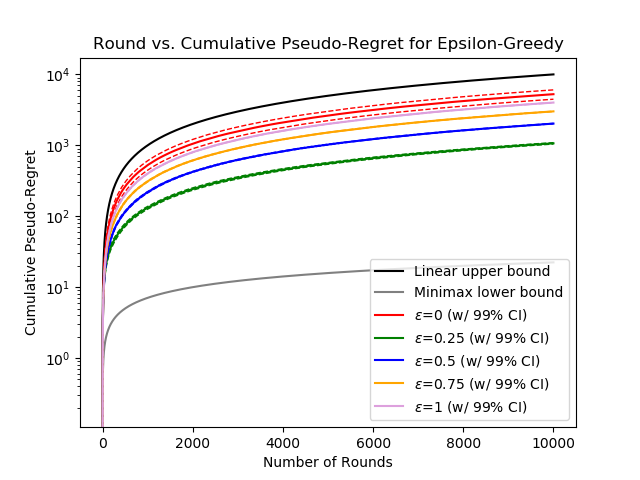
\includegraphics[width=\linewidth, height=0.75\linewidth]{epsilon-greedy.png}
\end{minipage}
\begin{minipage}[h]{0.5\linewidth}
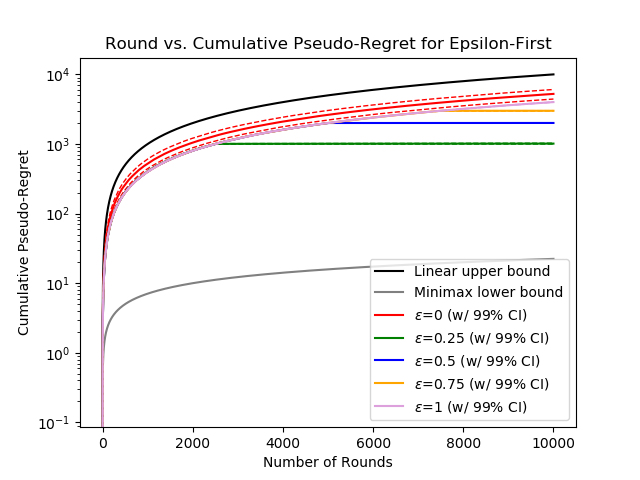
\includegraphics[width=\linewidth, height=0.75\linewidth]{epsilon-first.png}
\end{minipage}
\captionsetup{justification=centering}
\caption{Cumulative Regret vs Rounds for $\epsilon$-greedy and $\epsilon$-first.}
\label{fig:epsilon-greedy-first}
\end{figure}
Notice that both algorithms did very similar to each other and even the relative positions of the curves for the various epsilons were exactly the same for both algorithms. Furthermore, the graphs are very illuminating with respect to what is the optimal value of $\epsilon$, at least in our setting. Empirically, we clearly see that low exploration rates (or $\epsilon$) are preferable. This can be seen from the fact that an $\epsilon$ of 0.25 outperformed the one of $0.5$, and that one outperformed the one of $0.75$. Intuitively, this makes sense. Given that our setting does not have that many levers, the need for constant exploration is not that high. Even with a low $\epsilon$, given enough rounds, our algorithm is expected to have sampled the majority levers. Once this occurs, the algorithm will have a good approximate knowledge of which one is the best lever and the high exploitation rate (or $1-\epsilon$) will allow it to take advantage of that in many more occasions that in cases with higher $\epsilon$. Of course, if $\epsilon$ is too small (or as in our graph, it is zero), then exploration will not be done with enough consistency and this in turn will lead to less effective exploration and thus, higher regret. Finally, we notice that the worst case was when no exploration was done. This makes sense: the algorithm chose a random lever and pulled that one at every round. By simple probability, chances are the lever chosen was not the best one and hence, the algorithm will have high regrets. 

For empirically testing $\epsilon$-decreasing, we initialized $\epsilon=0.5$ (which evenly balances exploration and exploitation) and we tested for various decreasing factors $\delta$. Furthermore, we did this decrease every $N=1000$ rounds. The results are shown in Figure \ref{fig:epsilon-decreasing}.
\begin{figure}
\begin{center}
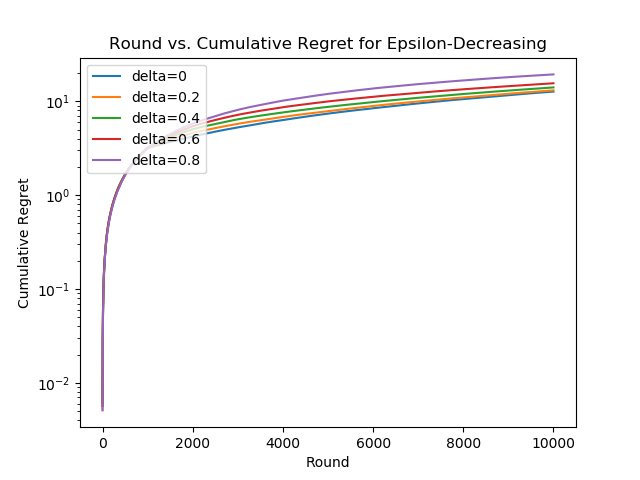
\includegraphics[scale=0.75]{epsilon-decreasing.png}
  \captionsetup{justification=centering}
  \caption{Cumulative Regret vs Rounds for $\epsilon$-decreasing with $\epsilon=0.5$ and $N=1000$.}
  \label{fig:epsilon-decreasing}
 \end{center}
\end{figure}
It can be seen that the lower the decreasing factor, the better the algorithm approximately performed. Intuitively, this makes sense for the following reason. Our initial $\epsilon$ is high and it is not modified until after 1000 rounds. It can thus be expected that by that round, the algorithm has explored enough to the point that it found a well performing lever. Hence, there is little need for more exploration and thus, substantially decreasing $\epsilon$ (or even setting it to 0 as in $\delta=0$), permits the algorithm to perform more exploitation.

\subsection{UCB and Thompson Sampling}

\textbf{Thompson Sampling Final Mean Pseudo Regret $105.12$, UCB Final Mean Pseudo Regret $753.12$}

Here we perform $10000$ rounds of experiment and we run the experiment $100$ times. We plot the upper bound and lower bound for UCB and Thompson Sampling. We also plot the mean pseudo-regret for both algorithms with $99$\% confidence interval.As the graph shows, the performance of UCB algorithm and Thompson Sampling algorithm fall between the theoretical upper bound and lower bound. Although the upper bound and lower bound are not very tight. Furthermore, Thompson sampling outperforms UCB algorithm by a significant margin despite the fact that both algorithms have the same theoretical lower bound and upper bound. These results show that theory can often provide very good qualitative information about performance of algorithms, but not very good quantitative information.

\begin{figure}[tb]
  \includegraphics[width=\linewidth]{Pseudo-Regret-Bounds.png}
  \captionsetup{justification=centering}
  \caption{Stochastic Reward Setting Pseudo-Regret Bounds}
\end{figure}

\subsection{Exp3 and Exp3.P Algorithms}

\begin{figure}[H]
\begin{minipage}[h]{0.5\linewidth}
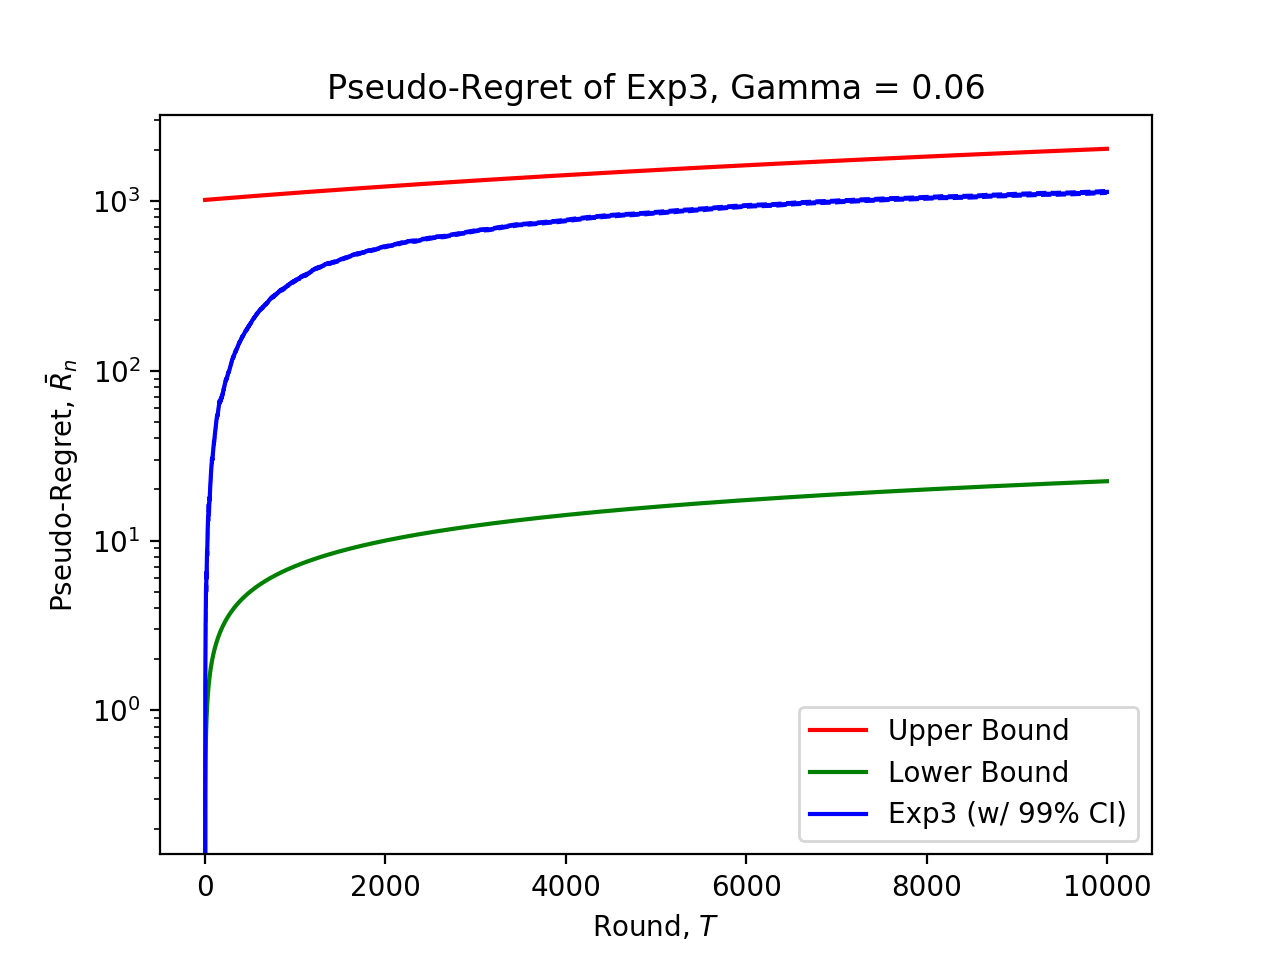
\includegraphics[width=\linewidth, height=0.75\linewidth]{exp3-1.png}
\end{minipage}
\begin{minipage}[h]{0.5\linewidth}
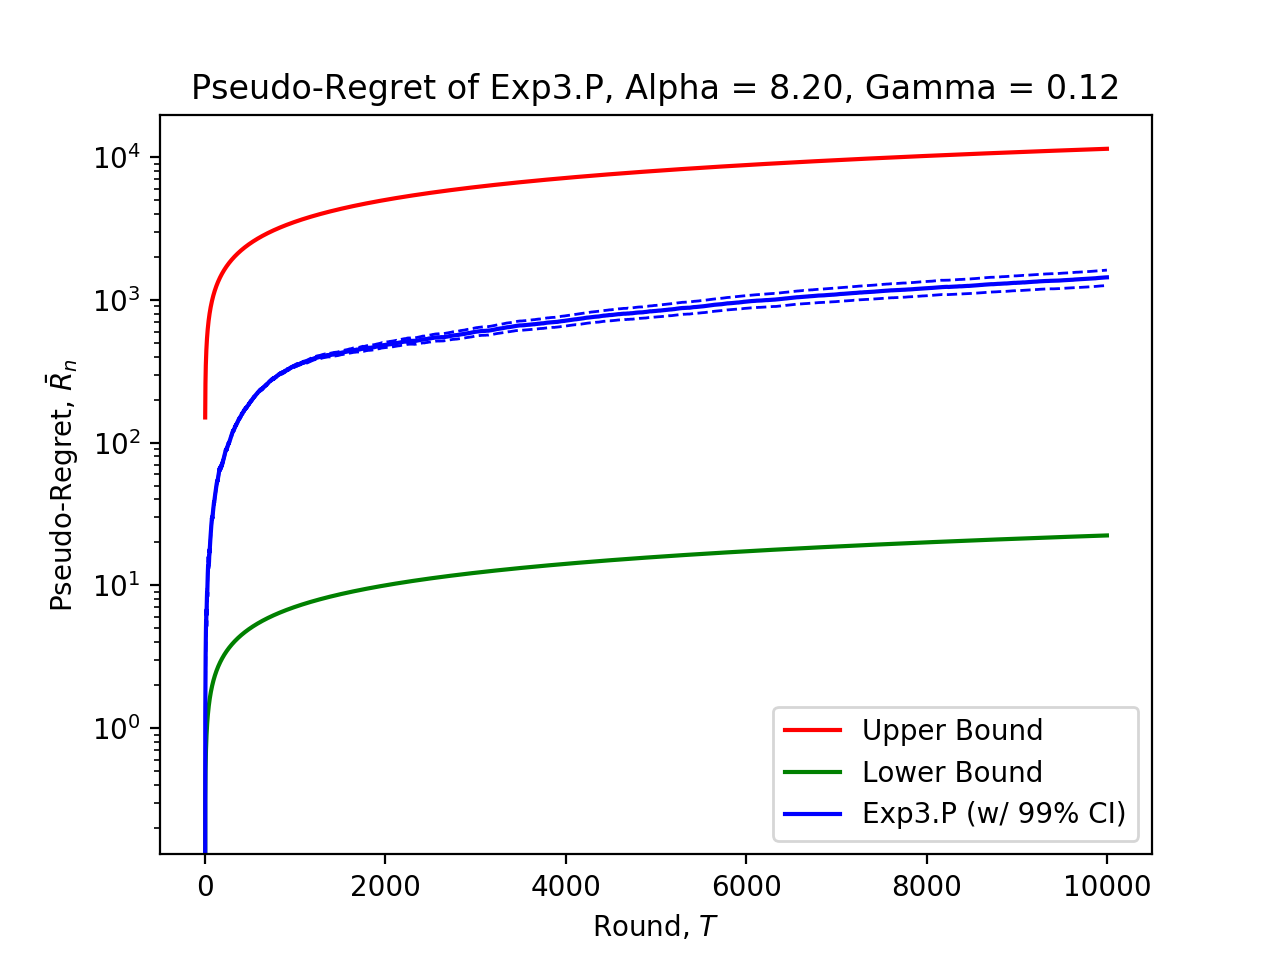
\includegraphics[width=\linewidth, height=0.75\linewidth]{exp3P-1.png}
\end{minipage}
\end{figure}

\section{Conclusion}

\newpage
\printbibliography

\end{document}